\chapter{Решение} \label{chapt3}

\section{Первая итерация} \label{sect3_1}

\subsection{Получение данных}
Для решения задачи классификации нейронной сетью требуется наличие данных для обучения. Датасетов с настоящей проблемой в открытом доступе не нашлось, поэтому данные пришлось получать вручную.

\begin{figure}[ht] 
  \center
  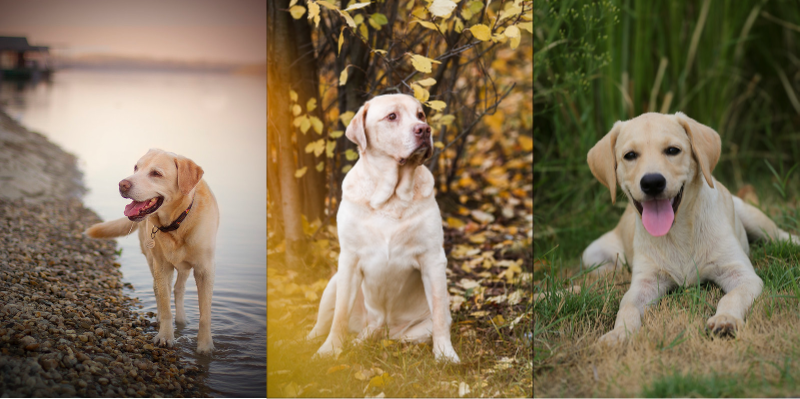
\includegraphics [width=\textwidth*2/3] {dogs-classes}
  \caption{Позы собаки, на которые классифицируются изображения: собака стоит, собака сидит и собака лежит} 
  \label{img:classes}  
\end{figure}

За основу был взят датасет OpenImageDataset[2] - набор изображений на более чем тысячу разных классов. Из него был взят подкласс Dog, в котором было 20000 изображений собак. Далее эти данные были размечены на Яндекс.Толоке. Каждое изображение было показано пользователю Толоки с вопросом “В какой позиции собака находится на этом фото”. Фотографии были размечены с пятикратным перекрытием, т.е. каждое изображение размечалось пять раз разными людьми.
На выходе получился скромного размера датасет, часть изображений в нём не подходили под постановку задач, но на выходе имелась информация о позе собаки, а также об ограничивающей рамке конечностей, с уклоном в будущее. Первой целью было поставлено научить нейронную сеть стабильно распознавать позу собаки.

\subsection{Проверка задачи на решаемость}

Перед тем, как загружать данные в нейронную сеть, их было решено предобработать. Вместе с комплектом данных из OpenImageDataset шла таблица с информацией о следующем:
\begin{itemize}
    \item Координаты ограничивающей рамки объекта
    \item Список объектов в кадре
    \item Флаг того что объект загорожен
    \item Флаг того что объект обрезан
    \item Флаг того что объект - рисунок объекта, а не фотография
    \item Флаг того что объект является группой объектов
    \item Флаг того что объект находится внутри другого объекта
\end{itemize}
В идеальном случае, все флаги должны быть равны нулю - то есть объект не загорожен, не обрезан и не рисунок. Но если применить все фильтры окажется что из 20000 изображений осталось всего 5000. При этом оказалось так, что флагами может быть отсеяно много годных изображений, но при этом могут остаться и обрезанные и загороженные собаки. В общем, это совсем неконсистентный результат. А вот что действительно могло сильно помочь, так это ограничивающая рамка.

\begin{figure}[ht] 
  \center
  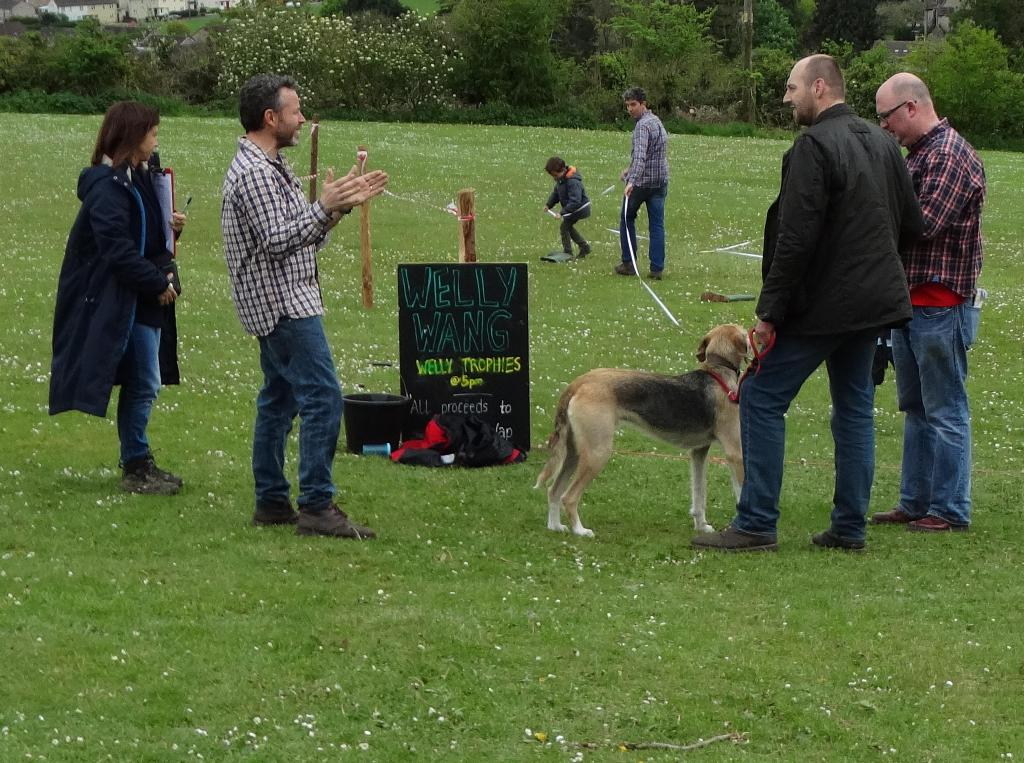
\includegraphics [width=\textwidth*2/3] {crop_helps}
  \caption{Изображение, которому сильно помогло бы обрезание по ограничивающей рамке собаки} 
  \label{img:crop_helps}  
\end{figure}

В теории, свёрточные нейронные сети инвариантны к расположению объектов в кадре, но вот к отвлекающим объектам они не инвариантны. Поэтому на практике обрезание по рамке собаки помогает значительно ускорить процесс обучения нейронной сети и сделать его более стабильным. К тому же, это избавляло множественных собак в кадре.

В итоге были предприняты следующие меры для улучшения работы системы.
\begin{itemize}
    \item Все изображения были обрезаны по ограничивающей рамке собаки. И это дало сильный прирост в качестве классификации, 55\% -> 65\% на 5 классах
    \item Дополнительно были размечены изображения, где собака видна плохо, и были удалены из выборки. Это сократило размер и без того маленькой выборки, не сильно улучшив данные, т.к. качество разметки на Толоке достаточно низкое.
    \item Добавлены аугментации обучающей выборки. Аугментации позволяют нейронной сети не запоминать обучающие данные точь-в-точь, что снижает её способность к переобучению.
    \item Проведена очистка изображений. Из обучающей выборки были исключены изображения с несколькими собаками и собаками, которых не видно целиком. Это дало самый ощутимый прирост, но обучающая выборка сократилась до недопустимо маленьких размеров. Добавлено около 3\% точности, 67\%->69\%
    \item Использование transfer learning (переносимость обучения) - все модели, которые использовались здесь, не обучались с нуля. Они обучались на нейронной сети, уже предобученной классифицировать 1000 классов ImageNet(другого открытого датасета с изображениями).
\end{itemize}

Но при всех стараниях, с каким бы фильтром не выбирались данные, как бы изображения не вырезались, какая бы глубина нейронной сети не выбиралась, точность нейронной сети никогда не превышала 67\%. Более того, из-за сильного дизбаланса классов, некоторые категории просто игнорировались классификатором в пользу более популярных. Для сравнения, в категории "собака лежит на спине" насчитывалось всего 400 изображений, против 4500 у категории стоящих собак. 

\subsection{Выводы на основе первой итерации}
Несмотря на трудности в сборе данных, и низкое качество классификации нейронной сети, был проведён анализ ошибок и выявлены следующие:
\begin{itemize}
    \item Для разметки данных надо использовать постоянных сотрудников, которым надо уделить время на то, чтобы разобраться с задачей. Низкая цена обучения не компенсирует многократные перекрытия в надежде найти статистическое среднее.
    \item Количество весов в нейронной сети и количество изображений в датасете должны быть линейно связаны. Хороший размер обучающей выборки для ResNet-34 (2.4 миллиона параметров) - строго от 100 тысяч изображений.
    \item Датасет надо балансировать по количеству изображений в каждом классе.
    \item В данных была огромная внутриклассовая разница между изображениями. У собак множество пород и размеров. Так как точность разметки не идеальна, нейронная сеть может запомнить что собака сидит, когда она чёрная, например. 
\end{itemize}{}

\section{Вторая итерация}

\subsection{Создание эталонного датасета} \label{subsect3_1_2}
Учитывая прошлые ошибки было принято решение собрать датасет заново, используя опыт, полученный при разметке первого.

Главные изменения заключаются в следующем:
\begin{enumerate}
    \item Датасет собирается итеративно по небольшим частям и выводы делаются сразу
    \item Размер каждого класса удерживается на одинаковом уровне
    \item Проводится учёт всех изображений, которые тяжело размечать
\end{enumerate}{}

В статье Amy Bearman и Cathering Dong \cite{Bearman2015HumanPE} указывается что нейронным сетям тяжело распознать позу, при наличии окклюзий, поворотов и переворотов, сильных перспективных искажений, и множественных объектов. В новом датасете было уделено особое внимание трудноклассифицируемым изображениям, поэтому они всячески избегались.

\begin{figure}[ht] 
  \center
  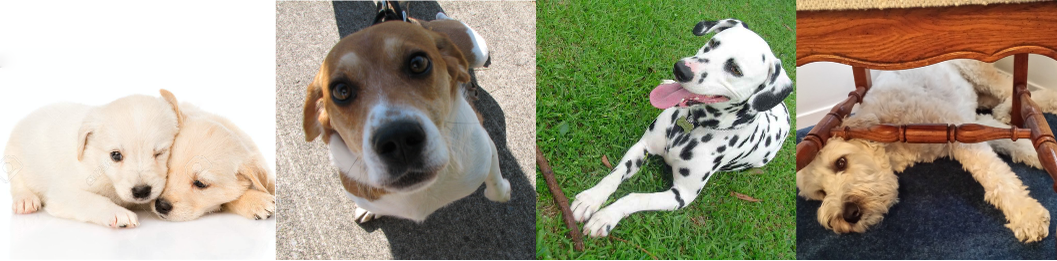
\includegraphics [width=\textwidth] {hazards_dogs}
  \caption{Позы, которые трудно определить: множественные объекты, перспективные искажения, повороты и окклюзии} 
  \label{img:hazards_dogs}  
\end{figure}

На этот раз источником изображений был Flickr. В нём содержится множество фотографий, который можно было фильтровать как по ориентации - только вертикальные, например. По породе - можно явно указать, что мы ищем Лабрадора Ретривера. Либо только снятые на телефон. В общем, сильно больше контроля при выборе фотографий.

Собирать фотографии заново было достаточно хорошим упражнением, но главной проблемой были огромные временные затраты на создание датасета даже с 300 фотографиями. Более того, из 80000 фотографий по тегу Лабрадор Ретривер, автором и его ассистентом было просмотрено 70000 из них. И уже из них были собраны 300 фотографий, по 100 изображений на целевой класс. 

\subsection{Попытка решить задачу на мини-наборе данных}
Количество данных накладывает сильные ограничения на выбор архитектуры нейронной сети. Разумеется, с 300 изображениями никаких популярных нынче архитектур не обучить. Но есть одна архитектура, которая смогла справиться с этой задачей. Это ShallowNet - нейронная сеть с одним свёрточным слоем.

\begin{figure}[ht] 
  \center
  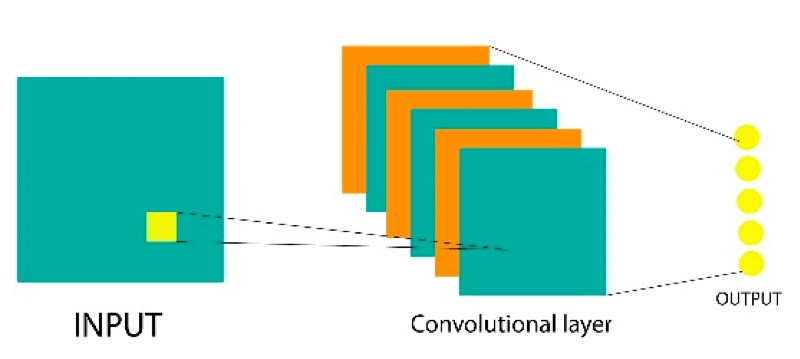
\includegraphics [width=\textwidth*2/3] {ShallowNet-architecture}
  \caption{ShallowNet - Минимально возможная архитектура свёрточной нейронной сети} 
  \label{img:shallownet}  
\end{figure}

Эта архитектура может показаться слишком простой, ведь есть и LeNet, в которой два свёрточных слоя. Но даже назначительное увеличение числа параметров сильно сказывается на переобучении. Все они бесконечно переобучаются, а валидационная точность выходит на плато в районе 50-60\%. Вот, для сравнения, то, с чем приходится иметь дело даже на такой простой архитектуре как LeNet:

\begin{figure}[ht] 
  \center
  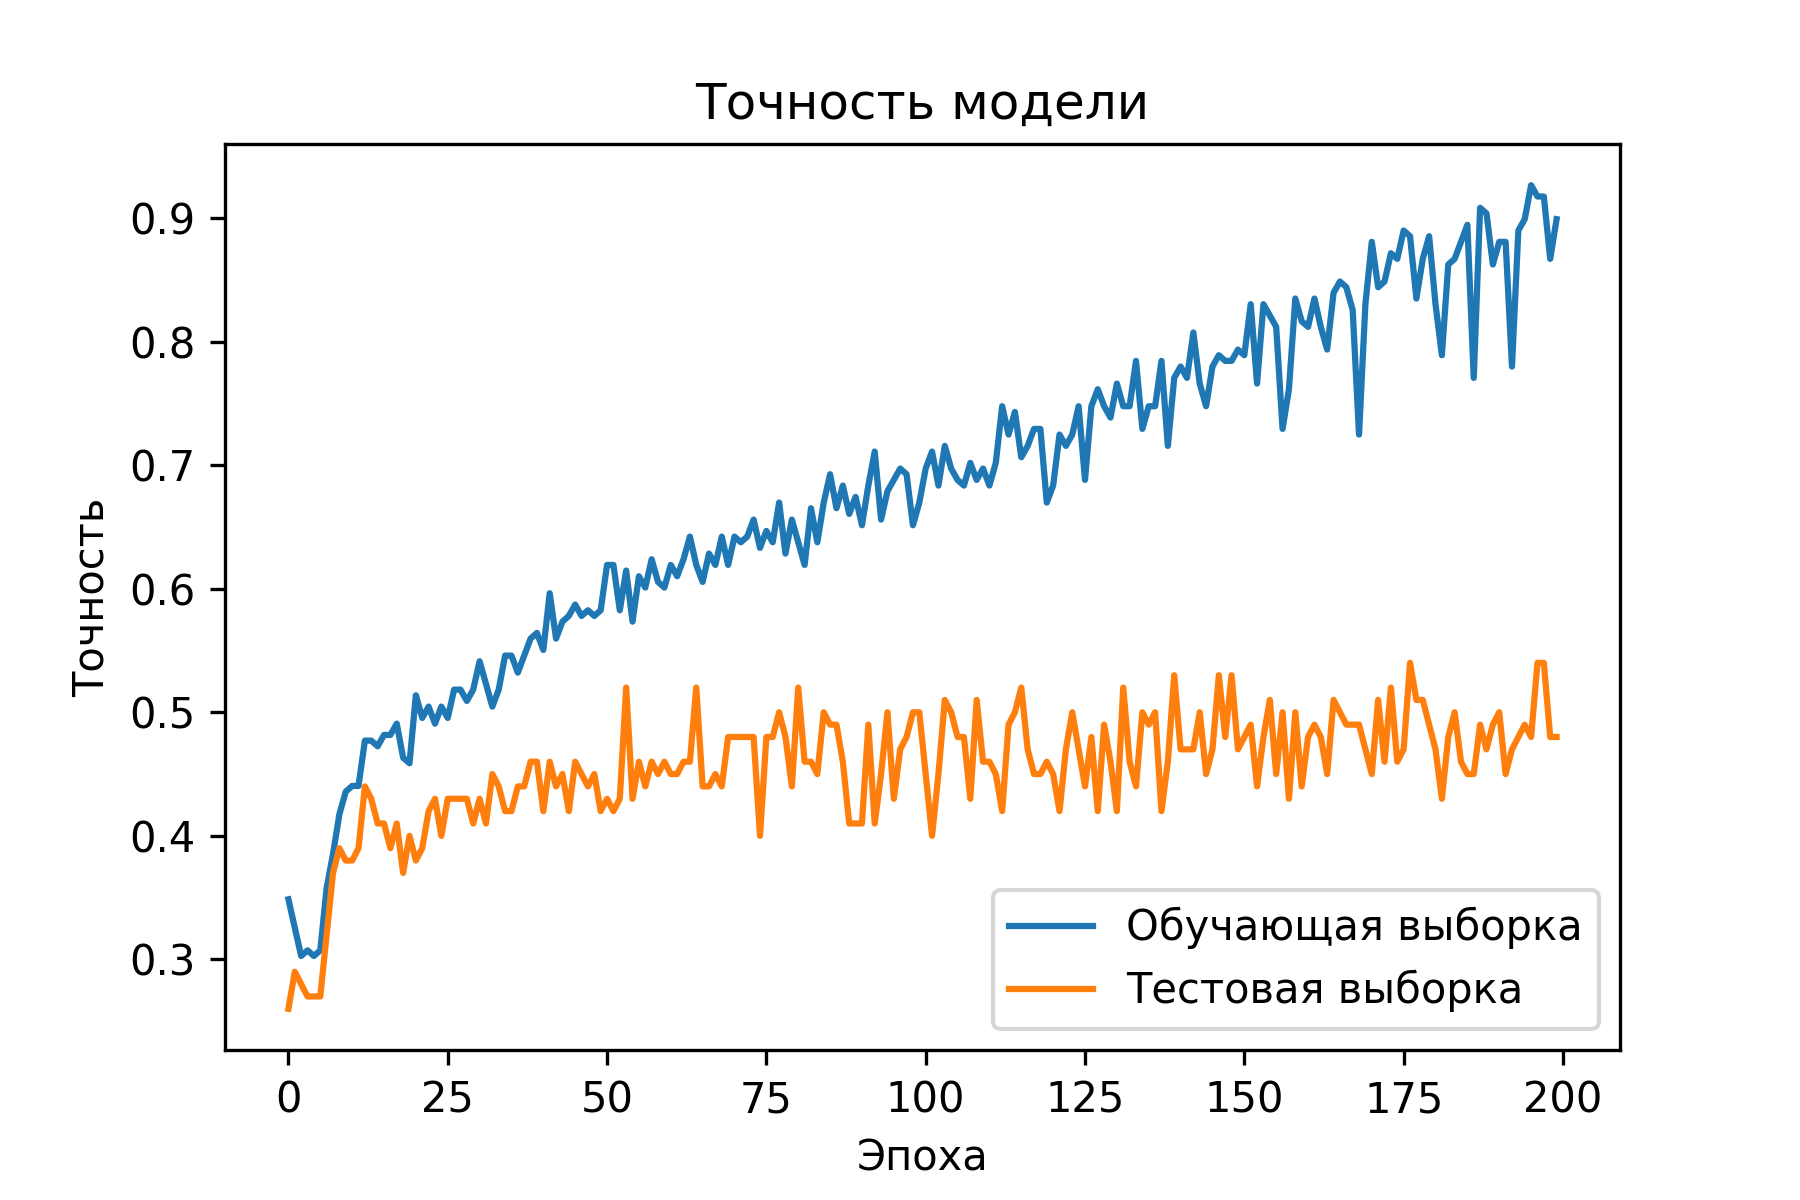
\includegraphics [width=\textwidth*2/3] {accuracy_over_epochs_lenet}
  \caption{Точность нейронной сети на обучающей выборке и на данных, которые нейронная сеть "не видит" при обучении. Можно заметить, тестовая точность выходит на плато ещё на 55 эпохе. Дальше идёт переобучение.} 
  \label{img:shallownet}  
\end{figure}

Таким образом, ShallowNet это единственная архитектура, на которой валидационная точность, т.е. точность на данных, которые не показывали нейронной сети при обучении, совпадала с теми же при обучении.

Результаты следующие:
\begin{itemize}
    \item При классификации «в лоб» достигается точность в 60\%
    \item При обрезании изображений по ограничительной рамке собаки, точность увеличивается до 68\%
    \item При использовании черно-белых изображений точность также возрастает до 68\%
\end{itemize}

Самым главным выводом из создания этого датасета является то, что даже такая маленькая сеть, как ShallowNet научилась распознавать данные с той же точностью, что и большая сеть. Большая сеть не заучивает никаких дополнительных знаний о позе собаки, кроме её геометрической фигуры. А стало быть, изображения должны быть хорошо различимы именно как геометрические фигуры. Кроме того, 68\% точности на такой элементарной архитектуре с таким сложным датасетом, это успех. 68\% на трёх классах это сильно выше случайного выбора. Случайный выбор дал бы 33\% точность.

\section{Обучение с частичным привлечением учителя} \label{sect3_3}
На основе результатов работы с маленьким, эталонным датасетом, автор попытался повторить успех на более крупном наборе данных с другой архитектурой. В итоге было принято решение просмотреть исходный датасет и повысить точность самих данных. Это достаточно просто, ведь в датасете, к этому моменту уже оставалось всего 5 тысяч фотографий. И исходя из качества в 70\%, присутствует около 15\% проблемных фотографий, которые достаточно удалить из коллекции чтобы повысить качество.

После недолгого просмотра фотографий было очевидно что эти фотографии слишком сильно отличаются от тех, что находятся в эталонном датасете. То есть, человек мог без проблем понять в какой позе животное изображено, но вот как геометрические фигуры, собаки не выстраивались в одну картину. И разумеется, чем пытаться рационализировать что нейронная сеть хорошо распознает, а что нет, проще спросить у неё самой.

\subsection{Разметка данных нейронной сетью}
Нейронная сеть может сильно помогать в разметке данных. Порой даже экономя время разметчиков в несколько раз. Главная идея здесь в том, что искать ошибки классификации нейронной сети намного проще, чем размечать данные самому. 
В наличии имелись следующие данные:
\begin{itemize}
    \item Датасет с собаками одной породы по 100 изображений на класс
    \item Повторно размеченные, "наиболее удачные"
    \footnote{Фотографии, на которых собака одна, и её ничто не загораживает} 
    5000 фотографий из 20000 доступных в OpenImageDataset.
    \item Все изображения с классом Dog в OpenImageDataset, их 20000, они не размечены.
\end{itemize}

Также была нейронная сеть, которая с 76\% точностью определяла сидят собаки, лежат или стоят. Такая точность никуда не годится, кроме одной цели. Этого достаточно чтобы узнать у самой нейронной сети какие фотографии ей легко различать, а какие нет.

Проклассифицировав весь датасет, были выбраны только изображения, в которых нейронная сеть не ошиблась, и уверенность была выше 99\%. Таких изображений из 5000 оказалось всего 400, причём 250 из них были те, где собака стоит. И всего 40, где собака сидит. Это очень сильный дизбаланс. Но зато все картинки, которые попали в этот крошечный датасет были идеальными. Собралась эталонная поза собак каждой позы.

% и здесь три подборки этих изображений по 20 штук на класс.

\begin{figure}[ht] 
  \center
  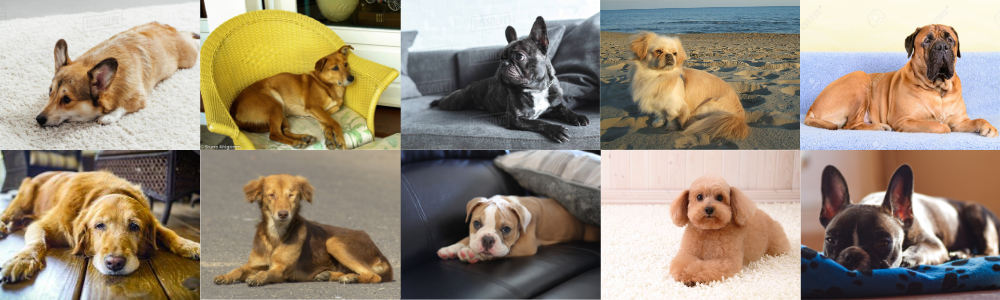
\includegraphics [width=\textwidth] {laying_perfect_dogs}
  \caption{Идеально лежащие собаки} 
  \label{img:laying_perfect_dogs}  
\end{figure}

\begin{figure}[ht] 
  \center
  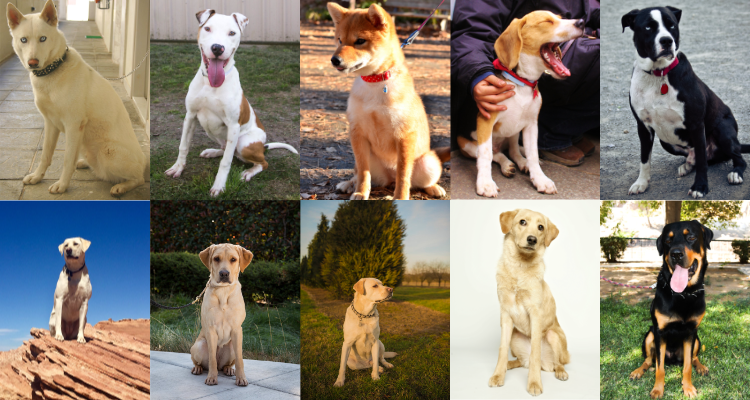
\includegraphics [width=\textwidth] {perfectly_sitting}
  \caption{Идеально сидящие собаки} 
  \label{img:perfectly_sitting}  
\end{figure}

\begin{figure}[ht] 
  \center
  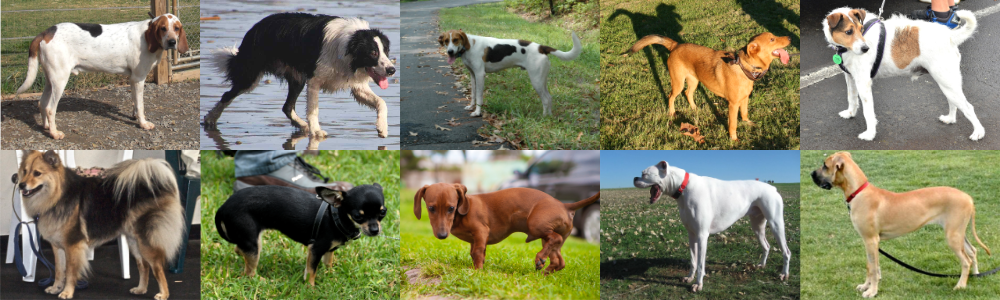
\includegraphics [width=\textwidth] {perfect_standing}
  \caption{Идеально стоящие собаки} 
  \label{img:perfect_standing}  
\end{figure}

Это как раз то, что было нужно. Все собаки были на достаточном отдалении от камеры и все их конечности были хорошо видны, т.е. не загораживали друг друга.

\subsection{Получение датасета}\label{sect3_3_1}

На основе увиденного, было принято решение собрать по этим эталонам больше собак, хотя бы по 500 на класс. В дальнейшем оказалось, что уверенность нейронной сети - относительный параметр. Классы, которые нейронная сеть легко классифицирует обладают достаточной дисперсией вокруг 100\% вероятности. На практике это означало, что для хорошо подготовленного класса сидячих собак, можно было опустить уверенность сети до 93\% чтобы получить схожую вероятность получить эталонные кадры.

Собственно, каждый класс датасета был дополнен лучшими его представителями до одинакового количества изображений на класс. После этого изображения прошли дополнительную чистку на наличие спорных изображений. Это позволило поднять количество изображений до примерно 300 на класс.

% спорное изображение, не понятно собака стоит или сидит.
\begin{figure}[ht] 
  \center
  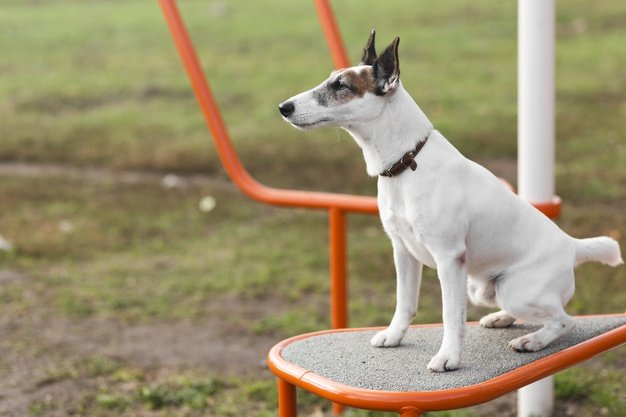
\includegraphics [width=\textwidth*2/3] {sit_or_stand}
  \caption{Спорное изображение, не понятно собака стоит или сидит.} 
  \label{img:laying_perfect_dogs}  
\end{figure}

Окончательно поставить точку в количестве данных позволил плохо размеченный OpenImageDataset. В нём все 20000 изображений были отклассифицированы, и лучшие его представители тоже были отобраны, а затем вручную проверены. В итоге это позволило добавить ещё по 200 изображений на класс до общих 500. Получается, выход достаточно небольшой: из 20000 изображений, частью нового датасета стали всего лишь 1500. (напомним, что предыдущие изображения были тоже взяты из этого датасета).
Недостающие изображения сидячих собак были дополнены 100 фотографиями сидячих лабрадоров из flickr. Маленький сет практически идеален, поэтому его можно брать без дополнительной проверки.

\subsection{Результаты на новых данных}\label{sect3_3_2}

Наконец, многообещающий новый датасет можно проверить на практике. Даже когда он ещё не до конца был собран, было ясно что его достаточно просто будет классифицировать.

Для классификации была взята модель MobileNet\cite{mobilenet} с изменённой головой классификации. Вместо ReLU на предпоследнем полносвязном слое использовалась функция активации ReLU, а также DropOut\cite{dropout} с вероятностью 20\% и BatchNorm \cite{batchnorm} - нормализация в пределах текущего фрагмента данных для обучения, с целью не допустить переобучения на столь маленьком наборе данных.

В результате получилась модель, которая с 96\% валидационной точностью классифицировала этот датасет. Благодаря мерам по регуляризации точность на отдельной выборке данных была схожа с точностью на обучающих данных.

\begin{figure}[ht] 
  \center
  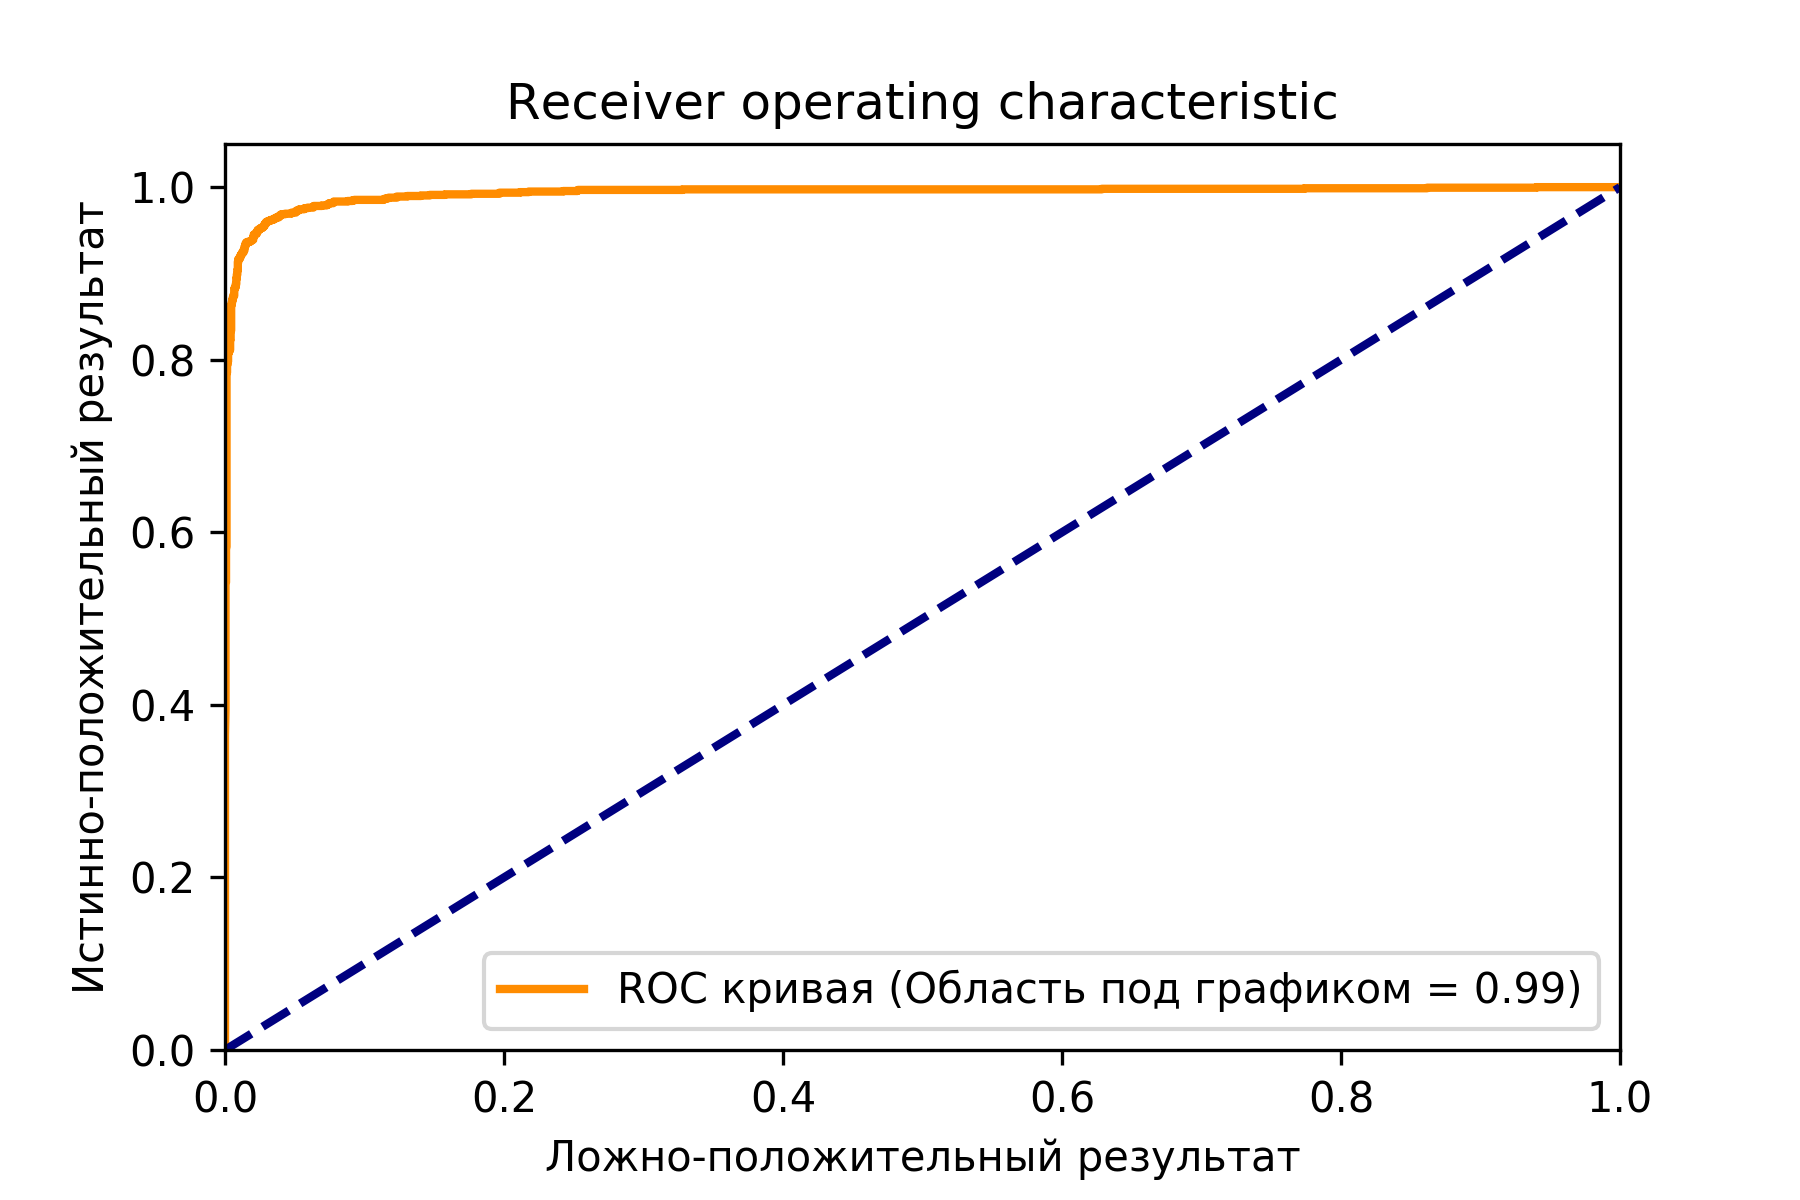
\includegraphics [width=\textwidth*2/3] {ROC_curve}
  \caption{Характеристическая кривая нового классификатора. Чем дальше рыжая кривая лежит от пунктирной линии, тем лучше.} 
  \label{img:ROC_curve}  
\end{figure}

Достоинства:
\begin{itemize}
    \item Есть датасет, на котором принципиально возможно обучить нейронную сеть
    \item Точность классификации достаточна для поставленной задачи
    \item Создан способ, позволяющий получить датасет любого размера. Требуется только однократная валидация человеком
\end{itemize}


Недостатки:
\begin{itemize}
    \item Нейронная сеть в состоянии работать только при удовлетворении множества условий, о которых будет рассказано далее
    \item Датасет не предусматривает наличие пограничных случаев - например, когда собака сидит, но не совсем обычным образом
    \item Не все позы собаки можно поделить на "сидит", "стоит" и "лежит". Собаки часто лежат на спине, на боку, лежат с поднятой головой итд. Собаки ещё бегут, прыгают и кружатся - все эти случаи не попадают под нашу классификацию.
\end{itemize}

Итог. Даже при наличии всех недостатков, лучше иметь систему, которая хорошо работает при известных случаях, чем ту, которая совершенно не работает при каждом случае. \cite{karpathy}


\subsection{Расширение датасета}\label{sect3_3_2}
Работать с маленькими датасетами на больших нейронных сетях крайне тяжело. Конечно, предобучение нейронных сетей на крупных наборах данных, таких как ImageNet, сильно помогает обучить глубокие слои и улучшает стабильность обучения, но 1500 изображений порой может не хватить даже для обучения "головы" нейронной сети.

Поэтому датасет постепенно расширялся в объёме по схожему принципу, указанному в предыдущей главе. На этот раз источником изображений стала группа «Shiba Inu Photography» в Facebook. В главном альбоме группы содержится 120 тысяч изображений, загруженными владельцами собак породы Шиба Ину.

Из загруженных 20000 изображений, в датасет попало 2205 изображений. То есть, как и изначально, всего 1 изображение из 10 оригинальных попадает в конечный датасет.

Итоговое количество изображений стало уже по 1500 изображений на класс, то есть 4500 изображений. Это уже сравнимо с часто используемыми датасетами как Animal Image Dataset(DOG, CAT and PANDA), в котором содержится по 1000 изображений собак, котов и панд. 


%Второй не такой красивый, но без ограничений (см.~листинг~\ref{list:hwplain}).
%\begin{ListingEnv}[H]
%    \begin{Verb}
%        
%        #include <iostream>
%        using namespace std;
%        
%       int main() //кириллица в комментариях
%        {
%            cout << "Привет, мир" << endl;
%        }
%    \end{Verb}
%    \caption{Программа “Hello, world” без подсветки}
%    \label{list:hwplain}
%\end{ListingEnv}